\documentclass[a4paper,14pt]{article}

\usepackage{comment} % Para comentar várias linhas ao mesmo tempo

%matemática
\usepackage{amsmath}
\usepackage{amssymb}

%diagramação
\usepackage{extsizes}
\everymath{\displaystyle}
\usepackage{geometry}
\usepackage{fancyhdr}
\usepackage{multicol}
\usepackage{graphicx}
\usepackage[brazil]{babel}
\usepackage[shortlabels]{enumitem}
\usepackage{cancel}
\usepackage{textcomp}
\usepackage{tcolorbox}

%tabelas
\usepackage{array} % Para melhor formatação de tabelas
\usepackage{longtable}
\usepackage{booktabs}  % Para linhas horizontais mais bonitas
\usepackage{float}   % Para usar o modificador [H]
\usepackage{caption} % Para usar legendas em tabelas
\usepackage{wrapfig} % Para usar tabelas e figuras flutuantes
\usepackage{xcolor} % Para cores do fundo de tabelas
\usepackage{colortbl} % Para cores do fundo de tabelas
\usepackage{upgreek} % Para inserir caracteres gregos

%tikzpicture
\begin{comment}
	\usepackage{tikz}
	\usepackage{scalerel}
	\usepackage{pict2e}
	\usepackage{tkz-euclide}
	\usetikzlibrary{calc}
	\usetikzlibrary{patterns,arrows.meta}
	\usetikzlibrary{shadows}
	\usetikzlibrary{external}
\end{comment}


%pgfplots
\usepackage{pgfplots}
\pgfplotsset{compat=newest}
\usepgfplotslibrary{statistics}
\usepgfplotslibrary{fillbetween}

%colours
\usepackage{xcolor}



\columnsep=2cm
\hoffset=0cm
\textwidth=8cm
\setlength{\columnseprule}{.1pt}
\setlength{\columnsep}{2cm}
\renewcommand{\headrulewidth}{0pt}
\geometry{top=1in, bottom=1in, left=0.7in, right=0.5in}

\pagestyle{fancy}
\fancyhf{}
\fancyfoot[C]{\thepage}

\begin{document}
	
	\noindent\textbf{6FMA154 - Matemática} 
	
	\begin{center}Fração geratriz: um método (Versão estudante)
	\end{center}
	
	\noindent\textbf{Nome:} \underline{\hspace{10cm}}
	\noindent\textbf{Data:} \underline{\hspace{4cm}}
	
	%\section*{Questões de Matemática}
	
	\begin{multicols}{2}
	    \noindent Um método para transformar dízima periódica em fração: \\
	    \begin{itemize}
	    	\item $0,\overline{5} = \frac{5}{9}$
	    	\item $2,\overline{3} = \frac{23 - 2}{9} = \frac{21}{9} = \frac{7}{3}$
	    	\item $0,1\overline{6} = \frac{16 - 1}{90} = \frac{15}{90} = \frac{1}{6}$
	    	\item $2,1\overline{3} = \frac{213 - 21}{90} = \frac{192}{90} = \frac{32}{15}$
	    \end{itemize}
		\noindent\textsubscript{--------------------------------------------------------------------------}
		\begin{enumerate} 
			\item Um cano tem por diâmetro 0,375757575... metro. Que fração do metro representa essa medida? \\\\\\\\\\\\\\
			\item Ache as geratrizes de:
			\begin{enumerate}[a)]
				\item 0,666... \\\\\\\\\\\\\\\\
				\item 3,222... \\\\\\\\\\\\\\\\
				\item 0,2444... \\\\\\\\\\\\\\\\
				\item $0,2\overline{137}$ \\\\\\\\\\\\\\\\
				\item 0,2333... \newpage
			\end{enumerate}
			\item Podemos dizer que $0,\dot{3} \cdot 0,\dot{5} = 1,\dot{5}$? Explique. \\\\\\\\\\\\\\\\\\\\
			\item Sejam $a = 2,555...$ e $b = 4,333...~$. Calcule:
			\begin{enumerate}[a)]
				\item $a + b$ \\\\\\\\\\\\\\\\\\
				\item $a - b$ \\\\\\\\\\\\\\\\\\
				\item $ab$ \\\\\\\\
				\item $\frac{a}{b}$ \\\\\\\\\\\\\\\\\\
			\end{enumerate}
			%35 a 42
			\item Qual é o 1 242º algarismo depois da vírgula na expansão decimal de $\frac{8}{41}$? \\\\\\\\\\\\\\\\\\
			\item Escreva a fração $\frac{143}{12}$ na forma de numeral decimal e classifique esse decimal. \newpage
			\item Coloque os seguintes números em ordem crescente: $19\%, (0,4)^2$ e $\frac{2}{11}$. \\\\\\\\\\\\\\\\\\
			\item Qual é o resultado da soma $x + y$ para $x = 0,989898...$ e $y = 0,131313...$? \\\\\\\\\\\\\\\\\\
			\item Calcule.
			\begin{enumerate}[a)]
				\item $4,302148302148... \cdot 3,5999...$ \\\\\\\\\\\\\\\\\\\\\\\\
				\item $(2,333...)^2 : 0,497497...$ \\\\\\\\\\\\\\\\\\\\
			\end{enumerate}
			\item Ao simplificar a expressão $\dfrac{\dfrac{1}{5} + \dfrac{1}{4} \cdot \dfrac{4}{9}}{0,\overline{88}}$, obtivemos:
			\begin{enumerate}[a)]
				\item 0,2121...
				\item 0,35
				\item 1
				\item 1,4
				\item 1,7555... \newpage
			\end{enumerate}
			\item Uma grande moldura de cobre foi produzida no formato a seguir. \\
			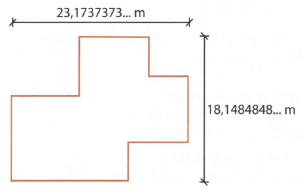
\includegraphics[width=1\linewidth]{6FMA154_imagens/imagem1} \\
			Os ângulos internos são todos retos. As barras de cobre usadas na construção custam R\$ 15,00 por metro. Qual foi o custo do material? Você pode usar uma calculadora para \textbf{ajudar} nas contas. \\\\\\\\\\\\\\\\\\\\
			\item Para $a = 0,7$, $b = 0,\overline{32}$ e $c = 1,\overline{3}$, calcule $a + b \cdot c^{-1}$ \\\\\\\\\\\\\\\\\\\\
		\end{enumerate}
		$~$ \\ $~$ \\ $~$ \\ $~$ \\ $~$ \\ $~$ \\ $~$ \\ $~$ \\ $~$ \\ $~$ \\ $~$ \\ $~$ \\ $~$ \\ $~$ \\ $~$ \\ $~$ \\ $~$ \\ $~$ \\ $~$ \\ $~$ \\ $~$ \\ $~$ \\ $~$ \\ $~$ \\ $~$ \\ $~$ \\ $~$ \\ $~$ \\ $~$ \\ $~$ \\ $~$ \\ $~$ \\ $~$ \\ $~$ \\ $~$ \\ $~$ \\ $~$ \\ $~$ \\ $~$ \\ $~$ \\ $~$ \\ $~$ \\ $~$ \\ $~$ \\ $~$
	\end{multicols}
\end{document}